%%%%%%%%%%%%%%%%%%%%%%%%%%%%%%%%%%%%%%%%%
% Structured General Purpose Assignment
% LaTeX Template
%
% This template has been downloaded from:
% http://www.latextemplates.com
%
% Original author:
% Ted Pavlic (http://www.tedpavlic.com)
%
% Note:
% The \lipsum[#] commands throughout this template generate dummy text
% to fill the template out. These commands should all be removed when 
% writing assignment content.
%
%%%%%%%%%%%%%%%%%%%%%%%%%%%%%%%%%%%%%%%%%

%----------------------------------------------------------------------------------------
%   PACKAGES AND OTHER DOCUMENT CONFIGURATIONS
%----------------------------------------------------------------------------------------

\documentclass{article}

\usepackage{fancyhdr} % Required for custom headers
\usepackage{lastpage} % Required to determine the last page for the footer
\usepackage{extramarks} % Required for headers and footers
\usepackage{graphicx} % Required to insert images
\usepackage{lipsum} % Used for inserting dummy 'Lorem ipsum' text into the template

\usepackage[T1]{fontenc} % Codificación de las fuentes utilizadas
\usepackage[spanish]{babel} % Español como idioma principal del texto (permite hyphenation de palabras al final de una línea)
\selectlanguage{spanish}
\usepackage{hyperref}
\usepackage{listings}

\usepackage[T1]{fontenc} % Codificación de las fuentes utilizadas
\usepackage[spanish]{babel} % Español como idioma principal del texto (permite hyphenation de palabras al final de una línea)


\usepackage{graphicx}
\usepackage{url}

\graphicspath{{Figures/}{Diagrams}{Chapters/}}  % Location of the graphics files (set up for graphics to be in PDF format)

\selectlanguage{spanish}

\setcounter{tocdepth}{1}

% Include any extra LaTeX packages required
\usepackage[square, numbers, comma, sort&compress]{natbib}  % Use the "Natbib" style for the references in the Bibliography
\usepackage{verbatim}  % Needed for the "comment" environment to make LaTeX comments
\usepackage{vector}  % Allows "\bvec{}" and "\buvec{}" for "blackboard" style bold vectors in maths
\hypersetup{urlcolor=blue, colorlinks=true}  % Colours hyperlinks in blue, but this can be distracting if there are many links.
\usepackage{hyperref}
% \usepackage[pdfauthor={Diego Martín Arroyo},
%             pdftitle={Diseño e implementación de un sistema de computación distribuida con
% Raspberry Pi, y estudio comparativo del mismo frente a otras soluciones},
%             pdfsubject={Memora del Trabajo de Fin de Grado},
%             pdfproducer={XeLaTeX with hyperref},
%             pdfcreator={XeLaTeX},
%             pdfkeywords={Computación Paralela, Sistema Distribuido, Raspberry}
%             ]{hyperref}
%% ----------------------------------------------------------------

%% --------------------------------------------------------------------------------------------------------------------------------
%http://tex.stackexchange.com/a/85218/76599
\usepackage{fancyvrb}
\usepackage[dvipsnames]{xcolor}

% redefine \VerbatimInput
\RecustomVerbatimCommand{\VerbatimInput}{VerbatimInput}% Inclusión de archivos de texto plano
{fontsize=\footnotesize,
 %
 frame=lines,  % top and bottom rule only
 framesep=2em, % separation between frame and text
 rulecolor=\color{Gray},
 %
 label=\fbox{\color{Black}data.txt},
 labelposition=topline,
 %
 commandchars=\|\(\), % escape character and argument delimiters for
                      % commands within the verbatim
 commentchar=*        % comment character
}

\usepackage{listings} % Requerido para la inserción de código
%Listings command

\usepackage{float}
\newcommand*\lstinputpath[1]{\lstset{inputpath=#1}}
\lstinputpath{Code/}

\newcounter{undefinedreferences}
\setcounter{undefinedreferences}{0}

\newcommand{\citationneeded}[1][None]{\stepcounter{undefinedreferences}\textsuperscript{\color{blue} [Citation needed: #1]}}

\newcommand{\checkreferences}{
\ifnum\value{undefinedreferences} > 0
\begin{center}
\immediate\write18{wget -O Figures/protester.png -nc http://imgs.xkcd.com/comics/wikipedian_protester.png}
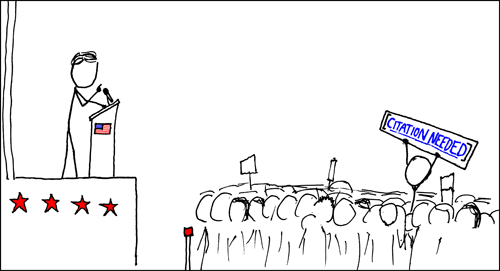
\includegraphics[width=\textwidth]{protester.png}\\
There are \arabic{undefinedreferences} undefined references
\end{center}
\else
No undefined references. Good!
\fi
}


%https://github.com/pads-fhs/LaTeX-Template-Thesis/blob/master/lststyles.tex
\lstdefinelanguage{JavaScript}{
  keywords={typeof, new, true, false, catch,%
    function, return, null, catch, switch, var,%
    if, in, while, do, else, case, break},
  ndkeywords={class, export, boolean, throw, implements, import, this},
  sensitive=false,
  comment=[l]{//},
  morecomment=[s]{/*}{*/},
  morestring=[b]',
  morestring=[b]"
}
\newcommand{\lstsetjavascript}{
  \lstset{
		language=JavaScript,
		breaklines=true,
		commentstyle=\textit,
		basicstyle=\ttfamily,
		keywordstyle=\bfseries,
		stringstyle=\ttfamily,
		showstringspaces=false,
		frame=single,
		tabsize=2
  }
}

\lstdefinelanguage{log}{
  keywords={typeof, new, true, false, catch,%
    function, return, null, catch, switch, var,%
    if, in, while, do, else, case, break},
  ndkeywords={class, export, boolean, throw, implements, import, this},
  sensitive=false,
  comment=[l]{//},
  morecomment=[s]{/*}{*/},
  morestring=[b]',
  morestring=[b]"
}
\newcommand{\lstsetlog}{
  \lstset{
		language=log,
		breaklines=true,
		commentstyle=\textit,
		basicstyle=\ttfamily,
		keywordstyle=\bfseries,
		stringstyle=\ttfamily,
		showstringspaces=false,
		frame=single,
		tabsize=2
  }
}

\lstloadlanguages{Java,XML, JavaScript, log}

\newcommand{\javascriptcode}[4]{
	\lstinputlisting[caption=#2,label=#1, firstline=#3, lastline=#4]{#1.json}
}

\newcommand{\logcode}[4]{
	\lstinputlisting[caption=#2,label=#1, firstline=#3, lastline=#4]{#1.log}
}

\usepackage[bottom]{footmisc} %The footnotes go at the bottom of t\usepackage{dtklogos}he page, instead next to the last line.
%Ajustes para Java
% \lstset{
% 	language=java,
%  	frame=single, % Un marco simple alrededor del código
%     basicstyle=\small\ttfamily, % Utilizar fuente true type pequeña
%     keywordstyle=[1]\color{Blue}\bf, % Funciones en negrita y azul
%     keywordstyle=[2]\color{Purple}, % Argumentos en morado
%     keywordstyle=[3]\color{Blue}\underbar, % Funciones personalizadas subrayadas en azul
%     identifierstyle=, % Nada especial acerca de identificadores
%     commentstyle=\usefont{T1}{pcr}{m}{sl}\color{Green}\small, % Los comentarios se renderizan en fuente pequeña verde
%     stringstyle=\color{Purple}, % Cadenas en morado
%     showstringspaces=false, % No se muestran los espacios entre cadenas
%     tabsize=5, % 5 espacios por tabulado
%     %
%     % Put standard Perl functions not included in the default language here
%     %morekeywords={rand},
%     %
%     % Put Perl function parameters here
%     %morekeywords=[2]{on, off, interp},
%     %
%     % Put user defined functions here
%     %morekeywords=[3]{test},\usepackage{dtklogos}
%    	%
%     morecomment=[l][\color{Blue}]{...}, % Line continuation (...) like blue comment
%     numbers=left, % Número de línea a la izquierda
%     firstnumber=1, % Número de línea comienza en 1
%     numberstyle=\tiny\color{Blue}, % Los números de línea son azules y pequeños
%     stepnumber=5, % Los números de línea van de 5 en 5
%     breaklines=true % Salto de línea si el texto no entra. See http://stackoverflow.com/a/1875803
% }

%\usepackage{xltxtra} % XeLaTeX logo. Yep, just that
%http://tex.stackexchange.com/a/73179/76599
\usepackage{metalogo}
%\usepackage{dtklogos} %BibTeX logo
\def\BibTeX{{\rm B\kern-.05em{\sc i\kern-.025em b}\kern-.08em
    T\kern-.1667em\lower.7ex\hbox{E}\kern-.125emX}}

\newenvironment{alignedDescription}[2][0pt]
  {\begin{list}{}%
    {\renewcommand\makelabel[1]{\textsf{\textbf{##1}}\hfil}%
     \settowidth\labelwidth{\makelabel{#2}}%
     \setlength\leftmargin{\labelwidth+\labelsep + #1}}}%
  {\end{list}}

\newenvironment{elements}
{\begin{quote}\itshape\centering\small}
{\end{quote}}

\newenvironment{cabstract}
{\begin{quote}\itshape\centering\small}
{\end{quote}}

%\usepackage[xindy]{glossaries}
%\newcommand{\chapterabstract}{1}{
%	\begin{center}
%	\small\textit
%	#1
%	\end{center}
%}

\usepackage{xcolor,colortbl}
\usepackage{float}
%----------------------------------------------------------------------------------------
%   NAME AND CLASS SECTION
%----------------------------------------------------------------------------------------

\newcommand{\hmwkTitle}{LED API} % Assignment title
\newcommand{\hmwkDueDate}{Viernes,\ 8\ de\ mayo\ de\ 2015} % Due date
\newcommand{\hmwkAuthorName}{Diego Martín Arroyo} % Your name

\graphicspath{{Figures/}}
%----------------------------------------------------------------------------------------
%   TITLE PAGE
%----------------------------------------------------------------------------------------

\title{\hmwkTitle}
\author{\textbf{\hmwkAuthorName}}
\date{\hmwkDueDate}

%----------------------------------------------------------------------------------------

\begin{document}

\maketitle

%----------------------------------------------------------------------------------------
%   TABLE OF CONTENTS
%----------------------------------------------------------------------------------------

\setcounter{tocdepth}{1}

\newpage
\tableofcontents
\newpage

\section{Introducción}

Uno de los componentes clave del sistema es su habilidad para facilitar el estudio de los sistemas distribuidos y la comprensión de los conceptos más básicos de este tipo de arquitecturas, así facilitar el desarrollo de aplicaciones distribuidas gracias a la intuitividad del sistema.

En este contexto surge la API de LEDs, un pequeño conjunto de sistemas \textit{software} y \textit{hardware} que permiten identificar de forma sencilla el comportamiento de un algoritmo distribuido en el sistema, apoyándose en la conmutación de una serie de diodos situados en cada placa. Dichos diodos están disponibles para el programador y pueden ser utilizados en una gran variedad de contextos.

\section{Hardware}

El conjunto de LEDs se sitúa en un circuito impreso que se conecta a la \textbf{Raspberry Pi} a través del puerto \textit{GPIO} (\textit{General Purpose Input-Output}), el cual provee de energía a los diferentes componentes.

\begin{figure}[H]
\centering
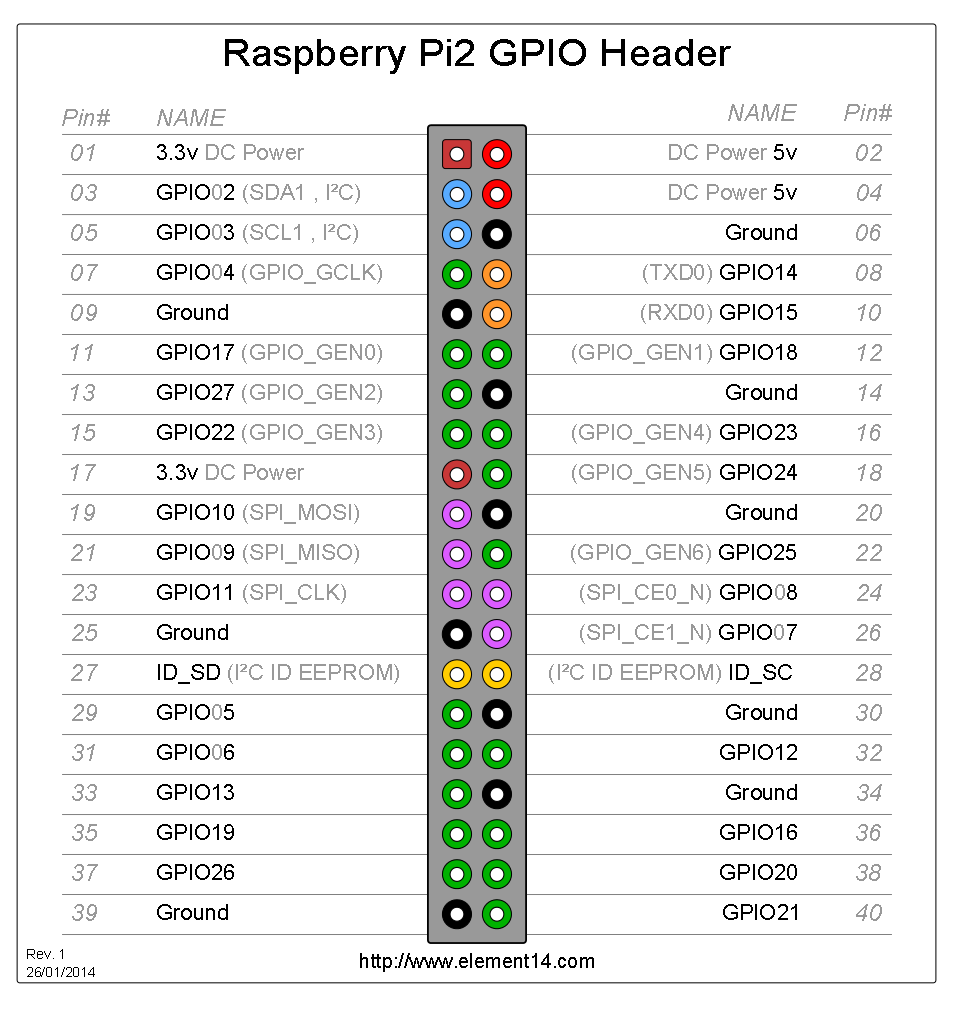
\includegraphics[width=0.4\textwidth]{GPIO_Pi2}
\caption{Puertos disponibles en la placa. El total de puertos asciende a 40, de los cuales 17 son de utilidad para la API}
\label{pi:gpio}
\end{figure}

La estructura de la placa divide claramente el conjunto de diodos disponibles en tres secciones, a detallarse en la sección \textit{software}:

\begin{itemize}
	\item \textbf{LEDs de estado} Accesibles únicamente por el administrador, permiten conocer el estado de la Raspberry (4 LEDs).
	\item \textbf{LEDs globales} Accesibles por el usuario, a través de un conjunto de aplicaciones definidas por el administrador, generalmente servicios globales (4 LEDs).
	\item \textbf{LEDs de usuario} Disponibles por completo para el programador una vez que ha conseguido acceso a los mismos (9 LEDs).
\end{itemize}

La placa se conecta directamente al puerto GPIO

\section{Software}

El software utiliza una API estándar para el manejo del encendido y apagado, limitándose a la gestión de permisos de acceso. Dicha acción se controla con los siguientes parámetros:

\begin{itemize}
 \item Dueño de la aplicación (root)
 \item Acceso garantizado a una serie de LEDs
 \item Acceso mediante \textit{tokens}
\end{itemize}

\subsection{Tokens}

La estructura de acceso a los LEDs de usuario se basa en la utilización de \textit{tokens} o testigos, objetos que otorgan el privilegio de uso de un recurso. En este caso se añade una restricción atípica: el tiempo de uso. La API otorga tokens siguiendo una estructura \textbf{FIFO}, otorgando acceso a una aplicación, mientras que el resto de las mismas se bloquearán a la espera de que el token sea entregado.

Sin embargo, este mecanismo no describe cómo se realiza la sincronización entre diferentes nodos de la infraestructura. Es deseable que cuando una aplicación obtenga un token de autenticación sea capaz de utilizar los LEDs en toda la infraestructura. Para ello se aprovecha \textbf{MarcoPolo}.

Una secuencia de interacción válida es la siguiente:

\begin{enumerate}
 \item Nodo 1 solicita acceso a LEDs
 \item Nodo 1 envía dicha solicitud a todos los nodos partícipes (o a un subconjunto definido, según el deseo del usuario), indicando la reserva del recurso, utilizando en la detección \textit{MarcoPolo}.
 \item Nodo 2 recibe el mensaje. Sin embargo, está ocupado atendiendo otra petición, por lo que la añadirá a una cola de espera. Nodo 1 bloquea su ejecución hasta que Nodo 2 libere el recurso. Dichas solicitudes se realizan en paralelo, por lo que el bloqueo se produce únicamente en uno de los hilos, no en el resto.
 \item Una vez que todos los nodos han cedido el acceso a la aplicación dada, se procede a la ejecución, que comienza a aprovechar la funcionalidad de los nodos.
 \item Cuando la aplicación termina, el privilegio de acceso se cede a la siguiente aplicación, repitiendo el proceso.
\end{enumerate}

La reserva se realiza en base a un LED en concreto, no al conjunto de todos ellos, por lo que en el caso de que cada usuario requiera únicamente un LED, podrían coexistir hasta 9 usuarios simultáneamente.
Dicho sistema garantiza la alternancia de varios usuarios, permitiendo establecer un sistema de turnos justo (basado en \textbf{FIFO}).



% \begin{figure}[H]
% \centering
% 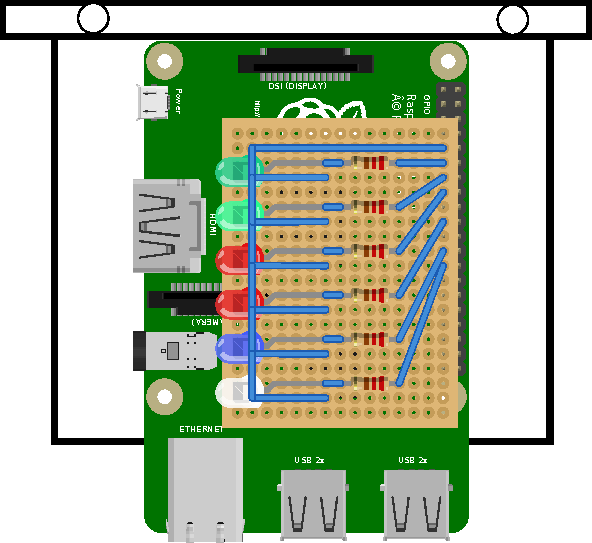
\includegraphics[width=0.4\textwidth]{placa}
% \caption{Diagrama de la placa con los LEDs}
% \label{pi:gpio}
% \end{figure}



 \label{Bibliography}
 \lhead{\emph{Bibliografía}}  % Change the left side page header to "Bibliography"
 \bibliographystyle{ieeetr}  % Use the "unsrtnat" BibTeX style for formatting the Bibliography
 \bibliography{led}  % The references (distcc) information are stored in the file named "distcc.bib"

\end{document}
